\providecommand{\main}{..}
\documentclass[\main/master.tex]{subfiles}
\begin{document}
\chapter{theoretical background}\label{chp:example-2}
\section{devices}

\subsection{Laser}
The laser is a high power coherent light source based on stimulated emmission with narrow spectrum. Inside a cavity Electron is excited to a higher energy level, and forced by photon with the correct wavelength to be absorbed emmiting coherent photon. The coherence allows focusing to a tight spot, and the spot staying collimated over long distances. 
\par
Continuous wave (CW) laser are lasing constant output power over time. Usually the power output is stable but has oscillations due to having several longitudinal modes causing nano second scale ossicilations, output power is steady when averaged over longer periods. Also, over long periods of time lasers have slight power oscillations due to temperture changes in the envirement.
%The laser diode cavity face is rectangular, because of fabrication constraints. The rectangular face is causing cylindrical aberration, which   

\subsection{Acousto Optic Modulator}
Acousto Optic Modulator (AOM), uses the acousto-optic effect to diffract and shift the frequency of light using RF waves. An oscillating electric signal drives a piezoelectric transducer to vibrate causing RF waves, the transducer attached to a material. This causes sound waves in the material, and periodic index modulation causing a Bragg grating. Incoming light scatters off the grating and due to Bragg diffraction comes at Bragg angle.
\begin{equation}
\theta_b = sin(\theta_b)\approx \frac{\lambda}{2n\Lambda} \label{eqn:energy-mass-equivalence-relation}
\end{equation} 
$\Lambda$ is the RF wavelength, $\lambda$ is the light source wavelength. 
\par
Since all parameters constant, modulation angle is constant, and possible modulation speed is nano seconds. Giving a stable fast modulation method for CW laser.



\subsection{Light Emitting Diode (LED)}
The light emitting diode (led) is a high power long lifetime light source semiconductor based. The led is emitting light when current flows through. Led could be modulated at up to 100MHz. The initial opening angle of a led source varies between 45 to 120 degrees. The emitted light is incoherent in width meaning it's hard to focus it to a point (not diffraction limited). The emitted light is incoherent in length causing wide band spectrum, although spectrum is sufficiently narrow to appear as a pure color to the human eye.
\par
The working principle is a semiconductor p-n junction with direct band gap. Meaning the lowest energy state above the band gap has the same momentum as the highest under the gap. In order to change energy state electron needs only to release energy equal to the band gap, which defines the wavelength $E_g = \frac{\hslash c}{\lambda}$. All possible energy gaps defines the spectrum, aproximatly gaussian around the wavelength. Forward voltage is applied causing electron injection and recombination with holes. The recombination is releasing energy in form of spontanious emmission photons. The modulation limitation is due to the electrons life time before recombination.
\par
The led power is proptional to the current flows through, Shockley diode equation for p-n junction defines the current relation to the diode voltage. In high enough values the power could be aproximated by liniar aproximation of the diode voltage.
\begin{equation}
P\propto e^{\frac{q}{kT}\cdot V_d}\label{eqn:energy-mass-equivalence-relation}
\end{equation}

\subsection{arduino}
Arduino is an open-source microcontroller board project used for building low cost and simple digital devices and circuits. Each microcontroller contains a microprocessor, controller, serial communication interface and is equipped with digital and analog input/output pins. The microcontrollers are controlled using C and C++ programming languages, and could be operated as stand alone or connected to the computer through serial communication. 
\par
There are multiple Arduino board models, we would focus on Arduino Mega 2560. The Arduino Mega 2560 is based on the ATmega2560, an Atmel 8-bit AVR controller. Also the board has 54 digital input/output pins of which 15 could be used as PWM outputs and a 16 MHz crystal oscillator (clock). In reality the arduino doesn't have analog output, to modulate the output Pulse Width Modulation technique is used.
\par
The controller is switching on/off the signal between the full Vcc of the board and off (5-0[V]), generating a square wave. The duration of time signal on is called the pulse width. The controller is able to modulate the pulse width, and change the ratio of time signal is on compare to off. The voltage is determined by the ratio of the time voltage is on compare to time voltage off, which is called duty cycle. 100\% duty cycle means the power is always on, 0\% duty cycle power is always off and 50\% duty cycle signal is on and off in equal times. 
%\\
\par

\begin{figure}[htbp]
	\centering
	\fbox{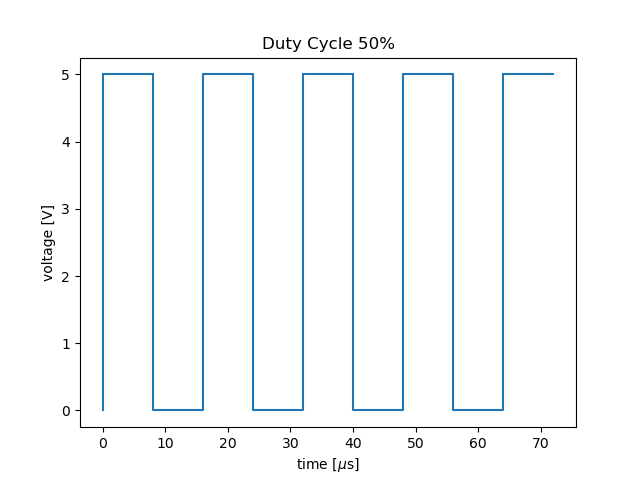
\includegraphics[scale=0.5]{\main/images/devices/duty50.png}}
	\caption[duty cycle 50\%]{50\% duty cycle  - signal is on and off equal times}
	\label{fig:duty50}
\end{figure}
Repeating that pattern fast enough results in an analog signal as if the signal is a steady voltage. This method is able to generate signals between the full Vcc of the board and off. The signal resolution is limited by the microcontroller resolution (8-bit). Due to the fast clock the of the arduino - the PWM analog modulation frequency is about 500Hz.
\par
\begin{figure}[htbp]
	\centering
	\fbox{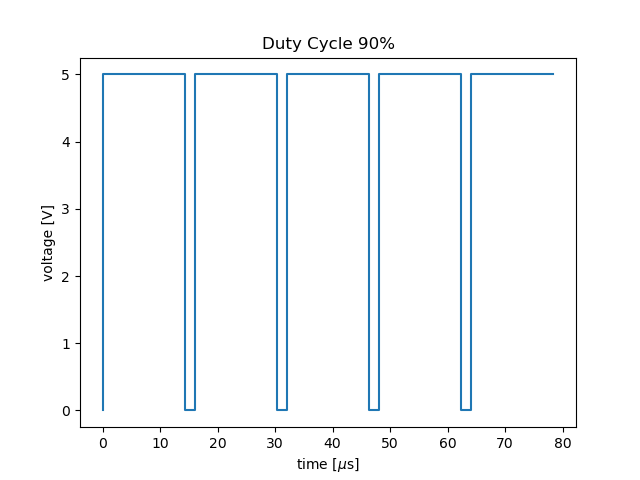
\includegraphics[scale=0.5]{\main/images/devices/duty90.png}}
	\caption[duty cycle 90\%]{90\% of the time signal on, equivalamt to 90\% of the full Vcc signal}
	\label{fig:duty90}
\end{figure}


\par
Using this method with a led connected, the led brightness could be modulated at about 2ms speed. Since the clock is connected to all PWM pins, if they all are in the same duty cycle, they are in sync. All pins are having a changing voltage, but they all have the same voltage, alowing to connect them in series and increase the output current, and the LED power. In conclusion this is a real-time controlled, fast-modulated, high power light source. 



\subsection{Light guides}
Light guides are pipes used for directed transmission of luminous energy.They are used to distribute light from the source to distant areas, they are made of thin filaments causing internal reflections. Light guides are used to illuminate small areas, regardless of the spectral characteristics of the light source. They mainly depend on the cross sections of entrance and exit and the length. Making them ideal to overcoming focusing problems, such as the LED uncoherent profile and large opening angle. 


\section{Radiation pressure}
Radiation pressure is pressure on the surface due to momentum exchange with electromagnetic field, including momentum of light. The light is at any wavelength which is absorbed, reflected, or emitted. The pressure is causing force on the surface, although the force is usually insignificant.
  
\par
The radiation pressure force depends on the angle of surface compare to electromagnetic field, surface intesity reflectance and absorbance, and the power of light hitting the surface $\Theta_i$ (radiant flux, measured in watts). There is coupling effitiency $\eta$ due to the light passing through a light guide or fiber, and size difference between the light spot size and the target size. A is the surface area, c is the speed of light. 
\begin{equation}
P_{incident} = \frac{\frac{\Theta_e}{A}cos^2(\alpha)}{c} = \frac{\eta\cdot \Theta_{source}\cdot cos^2(\alpha)}{{A\cdot c}} \label{eqn:energy-mass-equivalence-relation}
\end{equation}

Assuming the light Direction is perpendicular to surface, and angle is neglected. Also, the light variation over the surface is negligible.

\begin{equation}
F = P_{total}\cdot A = (P_{incident}+P_{emitted})\cdot A = 2\cdot P_{incident}\cdot A\label{eqn:energy-mass-equivalence-relation}
\end{equation}
\begin{equation}
F = \frac{2\eta\cdot\Theta_{source}}{{A\cdot c}}\cdot A = \frac{2\eta\cdot\Theta_{source}}{{c}} \label{eqn:energy-mass-equivalence-relation}
\end{equation}

%\begin{equation}
%\Theta_{source} = Q_e\cdot t = n\cdot\frac{\hslash c}{\lambda}\cdot t  \label%{eqn:energy-mass-equivalence-relation}
%\end{equation}
Assuming we have a power controlled light source with 1 watt maximum power and 40\% effietency we, we could inject forces of nano newton or less.  

 

\section{Vacuum Theory}
\subsection{Vacuum Chambers}
Vaccuum chamber is a metalic chamber with a vacuum pump which has a pressure lower than the atmospheric pressure (the atmospheric pressure is 760 [Torr]). Quality of vacuum is divided to ranges, according to the technology required to achieve it (such as CF, KF). Medium vacuum ($25-10^{-3}$ [Torr]), high vacuum ($10^{-3}-10^{-7}$ [Torr]) and ultra high vacuum ($10^{-7}-10^{-9}$ [Torr]). The main limitations to vacuum quality maintenance are leakage from the outside through the chamber and outgassing inside the chamber.
\par
Usually leaks and outgassing, are overcome by having the pump working constantly.Since, in this experiment, the pump is not working, due to the rotation noise. Leaks and outgassing both increases the pressure over time at a constant rate.  

\subsection{Leak Rate}
At any gas system, some gas would slowly leak over time and increase the pressure if not pumped out. The leak rate $Q_L$ is not a function of time, and resuls in a sustained increase of pressure P over time.
\begin{equation}
Q_L = \frac{\Delta P\cdot V}{\Delta t}  \label{eqn:energy-mass-equivalence-relation}
\end{equation}
The leak rate could also prevant the system from reaching initial low pressure (at some point the leakage would be equal to the pumping rate).
There is also diffusion of gas molecules, such as helium, which is insignifant when pressure is above $10^{-9}$. 

\subsection{Outgassing}
Outgassing is the desorption of gas molecules in vacuum (primarily water)  that were adsorbed or absorbed in the material. The outgassing occures over time and increases the pressure farther more. At low pressures, there are more gas molecules adsorbed on the chamber surface than floating in the chamber. The total surface area is more important than the volume for reaching low pressure. 
\par
The desorption rate $Q_{des}$ of the surfaces produces a gas yield that declines over time, dependent on the desorption density which is area specific. It could be assumed that after a given time $t>t_0$ the increase is liniar over time, typicaly $t_0$ assumed to be one hour.
\begin{equation}
Q_{des} = q_{des}\cdot A\cdot\frac{t_0}{t}  \label{eqn:energy-mass-equivalence-relation}
\end{equation}
Outgassing is minimized by selection of low vapor pressures materials such as stainless steel and glass. Since water is a significant source of outgassing, it is usually minimize by baking the chamber in high tempertures while the pump is running.

\subsection{Faraday Cage}
Faraday cage is a cage made by a continuous covering of a conductive material which is used to block electromagnetic fields. External electrical fields causes an electric charge distribution in the conductive cage without passing inside, which cancels the field's effect inside the cage. Faraday cage cannot prevent inside field caused by electric charges which are placed inside without touching the shield walls. Also, faraday cage blocks better high frequency magnetic field penetration, depending on the material skin depth penetration $\delta$.
\begin{equation}
\delta = \frac{2\rho}{(2\pi f)(\mu_0\mu_r)}     \label{eqn:mean-free-pass}
\end{equation}
Where $\rho$ is the material electric resistivity, and $\mu_r$ is the relative magnetic permeability. The cage cannot block stable or slowly varying magnetic fields from outside, the material skin depth determines the shield penetrating frequencies. Electric current decays exponentially with depth through the material, thicker shields attenuates lower frequency fields better. Vacuum chambers are usually made of a few mm thick stainless steel 316, making them faraday cages with a skin depth which could block magnetic frequencies higher than 10 KHz and reduce magnetic noise from lower frequencies.



\subsection{Viscous Flow}
The motivation to use vacuum is to reduce brownian motion and viscous friction caused by gas particles in the medium. Gas pressure at the medium is propotional to the number density of particles and inverse to the mean free pass of each particle.    
\begin{equation}
P = n\cdot k_B\cdot T  \label{eqn:ideal-gasses}
\end{equation}
\begin{equation}
I = \frac{k_B\cdot T}{\sqrt{2}\cdot\pi\cdot p\cdot d_m^2}     \label{eqn:mean-free-pass}
\end{equation}
Gas particle collide many times along it's way. The mean free path is the average distance the particle could pass between two collisions with other particles. Knudsen ratio could be derived from the term, ratio which is used to characterize types of gas flow compare to the pipe diameter.
\begin{equation}
K_n = \frac{I}{d}     \label{eqn:mean-free-pass}
\end{equation}

\subsection{Viscous Friction}
The friction caused by gasses is viscous friction, which is velocity dependenant. The velocity dependence is complicated, at very low speeds, gas resistance is approximately proportional to velocity. 

\begin{equation}
F_{drag} = -b\cdot v  \label{eqn:energy-mass-equivalence-relation}
\end{equation}

At the medium vacuum regime $0.01<k_n<0.5$ the flow is called Knudsen flow. The molecules do not interact and move in straight lines between points. If the vaccum chamber is having medium vacuum or higher, classical viscous friction of objects with gas particles inside the chamber could be neglected.









\subsection{Brownian Motion}
Brownian motion is a pattern of random particles fluctuations inside a fluid, a random walk with no preferential direction of flow. This pattern happens at thermal equilibrium in a given temperature (on average there is no linear and angular momentum). 
\par
Maxwell-Boltzmann distribution of molecular speed can extract the expression of average kinetic energy for a gas particle and the total brownian motion kinetic energie.
\begin{equation}
f(v) = 4\pi(\frac{m}{2\pi kT})^{3/2}v^2exp(\frac{-mv^2}{2kT})     \label{eqn:Maxwell_Boltzmann}
\end{equation}  
\begin{equation}
<E_k>=<\frac{mv^2}{2}> = \int_{0}^{\infty}\frac{mv^2}{2}f(v)dv =  \frac{3kT}{2}    \label{eqn:avrage_kinetic}
\end{equation}
\begin{equation}
E_k=N<E_k> \frac{3}{2}NkT    \label{eqn:total_kinetic}
\end{equation}
When system is in equilibrium, its kinetic energy is uniformly distributed among all its degrees of freedom. A macroscopic object in motion clearly is not in equilibrium. It has one degree of freedom (the center of mass motion) with far more energy than any other. If that degree of freedom interacts with others, the system will tend to move toward equilibrium. Energy will be transfered out of that one degree of freedom (so the object will slow down) and into all the others (so the object will become warmer).

That is all friction really is: the tendency of systems to move toward equilibrium when different degrees of freedom are allowed to interact with each other.

The Brownian motion of a particle is due to thermal energy. 

The Brownian motion kinetic energie is proptional to the number of particles. Vacuum reduces the pressure and number of particles, which reduces the energie.
\par
  











\section{Torsion Pendulum Theory}
\subsection{Torsional Pendulum}
Torsion Pendulum is an oscillator made of mass hung by a string from a fixed point so it could swing free. When the mass is displaced from equilibrium angle, the pedulum is having a liniar restoring tourqe, caused by the twisted string. The restoring tourqe is rotating the mass back to equilibrium position.


\begin{figure}[htbp]
	\centering
	\fbox{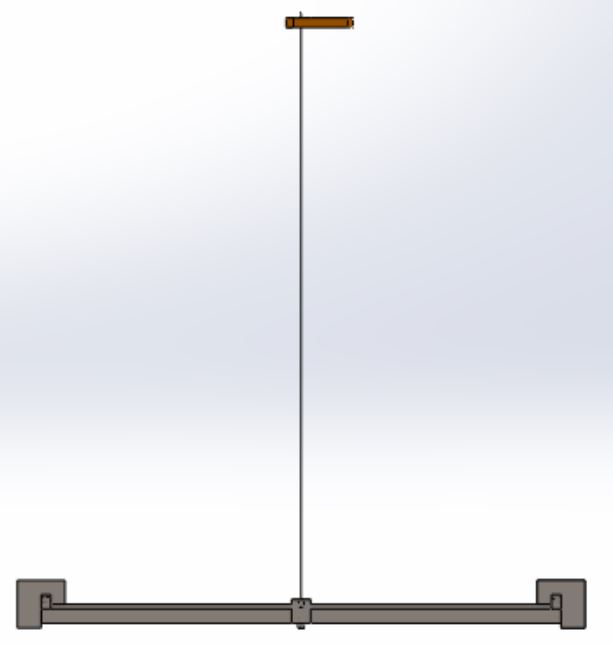
\includegraphics[scale=1.2]{\main/images/2 - theoretical background/torsion_pendulum.JPG}}
	\caption[pendulum]{a torsion pendulum}
	\label{fig:torsion_pendulum}
\end{figure}

Assuming a mass with a profile which could be estimated to a long thin rod. When displaced from equilibrium, there are two sources of torque; the displacing tourqe and a liniar restoring tourqe at opposite direction. At equilibrium, when balance stabilizes in a specific angle, the two sources of torque cancel out. With small angles the pendulum obeys Hooke’s law, when $L$ is the rod length.
\begin{equation}
\tau = -\kappa\theta = LF    \label{eqn:Hooke_law}
\end{equation}
The moment of innertia of a rod oscillating around a pivot.
\begin{equation}
I = \frac{ML^2}{12}     \label{eqn:moment_innertia}
\end{equation}  


The string torsion coefficient $\kappa $ could be estimated, assuming homogeneousity of a circular string. Where G is the material shear modulus, j is the circular second moment of area ($Jzz$) and $h$ is the string length.
\begin{equation}
\kappa = \frac{GJ}{h} = \frac{G}{h} \frac{\pi D^4}{32}    \label{eqn:torsion_coefficient}
\end{equation}
Note  $\kappa$ could also be found empirically by finding  the  oscillations period.
 


\subsection{Simple Harmonic Oscillator}
Harmonic oscillator is a second order system that, when displaced, experiences a liniar restoring force proportional to the displacement from equilibrium. Torsional pendulum is an angular harmonic oscillator (equivalent to the liniar case, instead of velosity and force, angular velosity and tourqe).
\par

If the restoring tourqe is the only tourqe acting, the oscillator is not driven or damped, called a simple harmonic oscillator. The tourqe is causing sinusoidal oscillations (simple harmonic motion) around the equilibrium angle. The time period and tourqe are determined by the physical constants of the pendulum. 
\begin{equation}
\tau = -\kappa\cdot\theta  = I\cdot\ddot{\theta}   \label{eqn:undamped_motion_equation}
\end{equation}
\begin{equation}
\theta(t) = \theta_{max}cos(\omega_0 t )    \label{eqn:undamped_motion_equation}
\end{equation}
\begin{equation}
\omega_0  = \frac{2\pi}{T} = \sqrt{\frac{\kappa}{I}}   \label{eqn:undamped_motion_equation}
\end{equation}

\subsection{Damped Oscillator}
If the system is also having damping (friction) which is proportional to the velocity, the system is called damped oscillator.


\begin{equation}
\tau_{drag} = -b\cdot\dot{\theta}   \label{eqn:friction_tourqe}
\end{equation} 
\begin{equation}
\tau = -\kappa\cdot\theta - b\dot{\theta}  = I\cdot\ddot{\theta}   \label{eqn:damped_motion_equation}
\end{equation} 
\begin{equation}
\ddot{\theta} + 2\xi\omega_0\dot{\theta} + \omega_0^2\theta = 0   \label{eqn:damped_motion_equation}
\end{equation}

The system damping ratio $\xi$ is the ratio between critical damping and the actual damping. The parameter determines the type of damping the system has, and the damping time of the system $\tau$. The damping ratio is a function of the damping coefficient $b$. Sytem could either be undamped, overdamped, critically damped or underdamped.
\begin{equation}
\theta(t) = Ae^{-\omega_0 t(\xi+\sqrt{\xi^2-1})} + Be^{-\omega_0 t(\xi-\sqrt{\xi^2-1})}    \label{eqn:damped_motion_equation}
\end{equation} 
\begin{equation}
\xi = \frac{b}{2\sqrt{I\kappa}} = \frac{actual}{critical}  \label{eqn:damped_motion_equation}
\end{equation}
\begin{equation}
\tau = \frac{1}{\xi\omega_0} = \frac{1}{\frac{b}{2\sqrt{I\kappa}}\sqrt{\frac{\kappa}{I}} }= \frac{2I}{b}  \label{eqn:damping_time}
\end{equation}
\begin{equation}
\theta(t) = Ae^{-\frac{t}{\tau}\cdot(1+\sqrt{1-\frac{1}{\xi^2}})} + Be^{-\frac{t}{\tau}\cdot(1-\sqrt{1-\frac{1}{\xi^2}})}    \label{eqn:damped_motion_equation}
\end{equation}
\begin{figure}[htbp]
	\centering
	\fbox{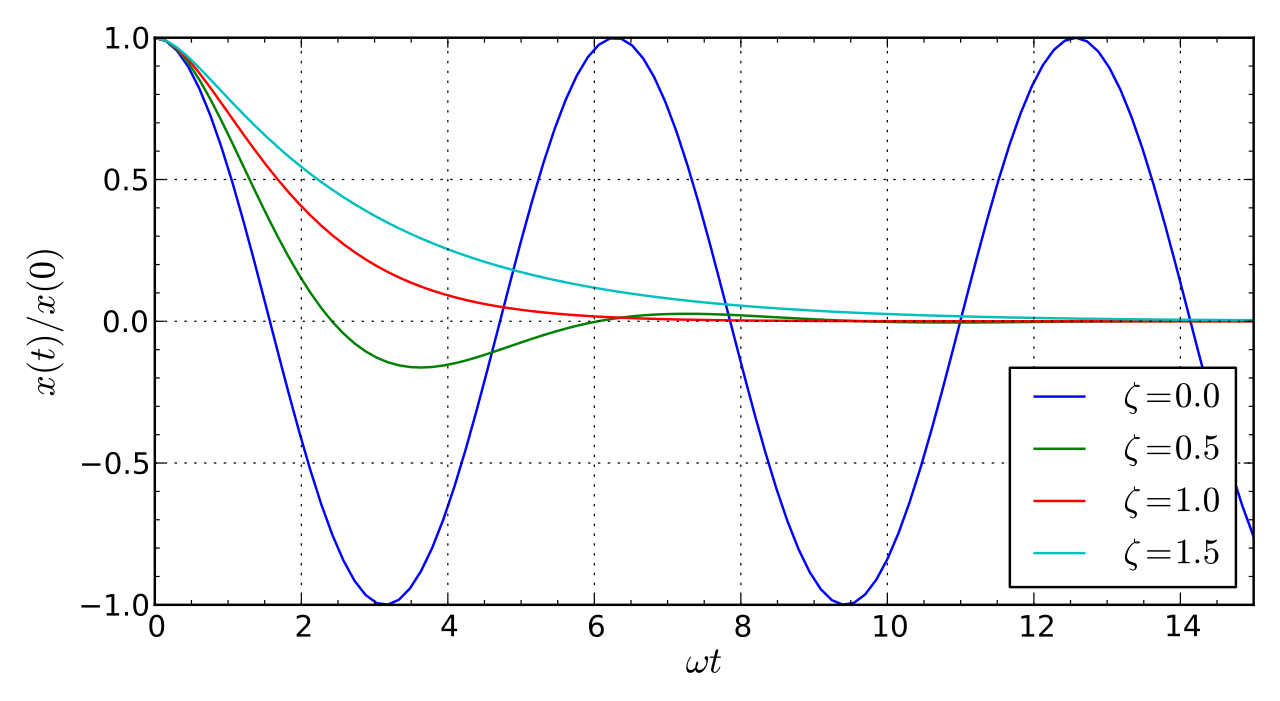
\includegraphics[scale=0.2]{\main/images/2 - theoretical background/damping.png}}
	\caption[damped]{damped oscillators; wikipedia}
	\label{fig:damped_oscillators}
\end{figure}



Undamped ($\xi = 0$); there is no friction and damping $b = 0$, harmonic oscillations without decay.
\begin{equation}
\theta(t) = \theta_{max}cos(\omega_0 t )    \label{eqn:undamped_motion_equation}
\end{equation}
Overdamped ($\xi > 1$); due to high friction, the system cannot oscillate and decays exponentialy to equilibrium position.
\begin{equation}
\theta(t) = Ae^{-\frac{t}{\tau}\cdot(1+\sqrt{1-\frac{1}{\xi^2}})} + Be^{-\frac{t}{\tau}\cdot(1-\sqrt{1-\frac{1}{\xi^2}})}    \label{eqn:overdamped_motion_equation}
\end{equation}
Critically damped ($\xi = 1$); due to high friction, the system cannot oscillate and decays exponentialy to equilibrium position. For a fixed $I, \kappa$, choosing $b$ to be at the critical damping value gives
the fastest return to equilibrium position. Although there is overshoot this is often a desirable property.

\begin{equation}
\theta(t) = \theta_{max}\cdot e^{-\frac{t}{\tau}}     \label{eqn:underdamped_motion_equation}
\end{equation}
 underdamped ($\xi < 1$); amplitude decreases in time due to the friction while oscillating with a lower frequency due to the damping. When the damping coefficient is small enough, the frequency change is neglected.
\begin{equation}
\theta(t) = \theta_{max}\cdot e^{-\frac{t}{\tau}}cos(\sqrt{1-\xi^2}\omega_0 t ) =  \theta_{max}\cdot e^{-\frac{t}{\tau}}cos(\omega t )    \label{eqn:underdamped_motion_equation}
\end{equation}
\begin{equation}
\omega = \omega_0\sqrt{1-\xi^2}\approx\omega_0    \label{eqn:underdamped_frequency}
\end{equation}

\subsection{Overshoot}
Overshoot is when output signal or function exceeds the target value. The response signal is not accurate compare to target.In controll theory there are two wanted conflicting properties; an accurate response (small overshoot), and small risetime (fast response). 
\par
Overshoot is usually measured in percentage overshoot (PO). For second order systems, such as damped oscillators PO is a function of the damping ratio $\xi$. 


\begin{equation}
PO = 100\cdot e ^{\frac{-\xi\pi}{\sqrt{1-\xi^2}}} = \frac{output-target}{target}   \label{eqn:percentage_overshoot}
\end{equation}
 



\iffalse
https://ocw.mit.edu/courses/mathematics/18-03sc-differential-equations-fall-2011/unit-ii-second-order-constant-coefficient-linear-equations/damped-harmonic-oscillators/MIT18_03SCF11_s13_2text.pdf

https://www.sciencedirect.com/topics/engineering/underdamped-system#:~:text=When%20the%20damping%20ratio%20is%20between%200%20and%201%20(i.e.,is%20an%20exponential%20decay%20line.


\subsection{Driven Oscillator}
If the damped oscillator system is further affected by an external time-dependent tourqe $\tau(t)$,  the system is called driven oscillator.
\begin{equation}
\tau(t) -\kappa\cdot\theta - b\dot{\theta}  = I\cdot\ddot{\theta}   \label{eqn:driven_motion_equation}
\end{equation} 
\begin{equation}
\ddot{\theta} + 2\xi\omega_0\dot{\theta} + \omega_0^2\theta = \frac{\tau(t)}{I}   \label{eqn:damped_motion_equation}
\end{equation}
\fi



\section{PID Controller}
\subsection{PID Controller Feedback}
proportional–integral–derivative controller (PID controller) is a feedback based control system. The control loop is used for time continuouse control of a process, so the process output (measured process variable) would be close to a defined set point.
\par
PID controller continuously calculates error value, which is the distance of the measured process variable from the defined set point. The feedback applies an external correction to the process, called control variable. The control variable is based on a proportional, integral and derivative gain to the error. Proper tuning of a PID enables an accurate automated correction to a controled process. The PID concept is used widely in applications requiring accurate automated control.
\par
\begin{figure}[htbp]
	\centering
	\fbox{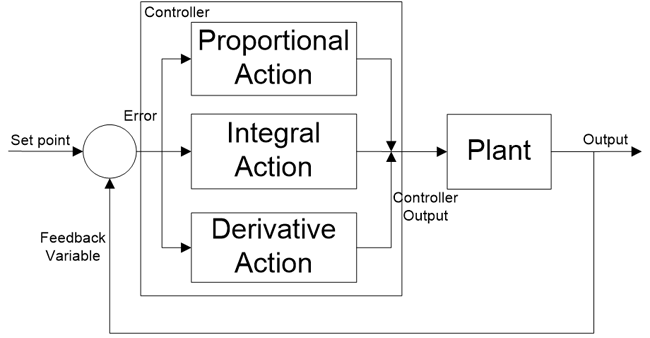
\includegraphics[scale=0.2]{\main/images/2 - theoretical background/PID.png}}
	\caption[PID]{PID controller feedback loop; from wikipedia}
	\label{fig:PID_scheme}
\end{figure}


\par
The error and the error's integral and derivate are calculated continuously. The control is having three tuning parameters; $P, I, D$, the feed back correction is modulated by the tuning parameters value. Each parameter is assigned to a gain (proportional, integral and derivative). The response (control variable) is a weighted sum of the control terms. Over time the controller attempts to minimize the error $e(t)$ by adjusting the control variable $u(t)$, which is the PID output.
\begin{equation}
u(t) = K_Pe(t)+K_I\int_{0}^{t}e(t)+K_D\frac{de(t)}{dt}   \label{eqn:PID_eq}
\end{equation}


P is proportional to the current error value $e(t)$. When error is large and positive, proportional output would be proportionately large and positive.
\par
I is proportional to past error value's integration. The response of the cumulative value could eliminate residual errors, such as signal offset.
\par
D is proportional to error current change rate, by calculating the derivative. The response of the change rate could eliminate more rapid changes.
\par
The optimal control function is achieved by balancing the responses. The tuning constants depend on the characteristics of the specific procces. The response must be tuned for each control application.  

\subsection{Damped Oscillator}
PID controller can continuously calculates error value of an oscillator, to damp it to zero. If the defined set point is set to zero, the error is the measured process variable. The PID acts as friction, gradually working when the ossicilations are at the maximum speed to slow them down, and remove the tourqe energy.
\begin{equation}
e(t) = \theta(t) = \theta   \label{eqn:error}
\end{equation}
\begin{equation}
\tau_{PID} = -\gamma\cdot\dot{\theta}   \label{eqn:friction_tourqe}
\end{equation}
The sytem is a damped oscillator, with an external force correction, which inserts tourqe to the oscillator.
\begin{equation}
\kappa\cdot\theta - \gamma\cdot\dot{\theta}  + I\cdot\ddot{\theta} = 0   \label{eqn:damped__pid_motion_equation}
\end{equation}
\begin{equation}
\gamma\dot{\theta}  = Fr   \label{eqn:damped__pid_motion_equation}
\end{equation}

\begin{equation}
\dot{\theta} = \omega_0\theta_{max}sin(\omega_0 t +\phi)    \label{eqn:undamped_motion_equation}
\end{equation}
\begin{equation}
\dot{\theta}_{max} = \omega_0\theta_{max} = \theta_{max}\cdot\frac{2\pi}{T}    \label{eqn:undamped_motion_equation}
\end{equation}
\begin{equation}
\gamma  = \frac{F_{max}r}{\dot{\theta}_{max}} =\frac{F_{max}rT}{\theta_{max}2\pi}    \label{eqn:damped_pid_motion_equation}
\end{equation}
\begin{equation}
\tau =  \frac{2I}{\gamma}  \label{eqn:damping_time}
\end{equation}
The PID damping depends on the initial oscillations angle. If the angle is too large compare to the inserted force, the system is extremly underdamped and the PID affect is neglected. The damping time $\tau$ would be infinite and the system would keep on ossicilating.

\subsection{Damping}
Using PID control does not guarantee optimal control or stability. The control system is aiming to achieve critical damping of the process. Well tuned control would a reach the desired set point fast and accurate, and also apply over time the nesseary corrections to resist external forces trying to move variable from the set point.
\par
The controller response is its response to error. How much does the sytem overshoots a setpoint and the system oscillations. When controller gains are too high, instead of critical damping there is overdamping causing overshoot, due to the high gain the overshoot response overshoots to the other side, causing driving of the system.





\section{Gravity Measurement}

\subsection{Gravitational Field}
Newton law of universal gravitation states that every point mass attracts every other point mass in the universe.
\begin{equation}
\overrightarrow{F}(r) = \frac{GMm}{r^2}\hat{r}    \label{eqn:gravitation_force}
\end{equation} 
The force is acting along the intersecting line, proportional to the product of the masses and inverse to the square of the distance between the centers. Since it is inverse to the distance square means the force is very weak. For example the force between two cubes 1 kg each 1 meter away would be $\overrightarrow{F} = 6.67\cdot10^{-11} [N]$.
\par
Gravitational field of a mass is a vector field consisting at every point a vector pointing directly towards the particle. The magnitude of the field at every point is calculated by applying the universal law, the force per unit mass. 
\begin{equation}
\overrightarrow{G}(r) = \frac{\overrightarrow{F}(r)}{m} = \frac{GM}{r^2}\hat{r}    \label{eqn:gravitation_field}
\end{equation}
The field caused by a mass at a specific point is measured by measuring the gravitational force. The gravitational force caused by a small known mass test mass $m$ relative to the mass $M$. Test mass $m$ much smaller than mass $M$ ensures that there is a negligible influence on the behavior of $M$.  



\subsection{Cavendish Experiment}
The Cavendish experiment, performed in the 17th century, was the first experiment to measure the gravitational force between masses. The apparatus which is constructed by a torsional pendulum is still used to measure accurately gravitational forces. Assuming no friction or other damping force (simple harmonic oscillator) when a mass is interduced, there are two sources of torque in the system; tourqe by the mass gravitational force, and restoring tourqe caused by the wire torsion. Since gravity is a weak force the torsional pendulum obeys Hooke’s law (small angles). At equilibrium, when balance has been stabilized at an angle $\theta$, these two tourqes are canceled out.
\begin{equation}
\overrightarrow{\tau} = \kappa\theta = LF = L\frac{GmM}{r^2}    \label{eqn:gravitation_tourqe}
\end{equation}


\subsection{Gravity Sensing}
The field at a specific point is the super position of fields point value, of fields caused by any mass in space. Measuring accurately the gravitational field caused by a mass, with a known test mass, the mass weight or distance could be estimated. In order to filter out the other gravitational fields, caused by masses around, the measurement is measuring the difference from a baseline state.
\par
Usually the measurement is with a frequency. The test mass is moving in different frequencies (not moving is zero frequency). The masses around are not moving, and are filtered out.
\par
The angle caused by thr gravitational field is measured at each of those frequencies, measuring the energy spectral density $[\frac{rad}{\sqrt{Hz}}]$.
In the measurement system different noises have different frequencies. By integrating over long time measurement noises are reduced. The signal to noise ratio (SNR) is the limiting factor for the sensetivity of a measuring system. In higher frequencies integration is faster, causing less noises and higher SNR.
The SNR dependency on frequency cause difficuties measuring gravitational fields at low frequencies.




\section{Thermodynamic temperature}

\subsection{shotnoise}



\end{document}







